\section{Vorbereitung}

\noindent{\large Arbeitsaufteilung:\par}
\begin{table}[htb]
\centering
\caption{Arbeitsaufteilung in der Gruppe}
\label{Arbeitsaufteilung}
\begin{tabular}{c|ccc}
\toprule
Aufgabe & Lucas & Aleksandra & Timo\\
\midrule
Motivation &  & x & \\
Literaturrecherche &  &  & x\\
1.2 Filterschaltungen & x & x & x\\
1.3 Addierschaltung & x & x & x\\
Dokumentation & x & x & x\\
Diskussionen & x & x & x\\
Bericht \& Spice & x &  & \\
\bottomrule
\end{tabular}
\end{table}

\noindent{\large Genutzte Materialien:\par}
\begin{table}[htb]
\centering
\caption{Genutzte Materialien}
\label{Arbeitsaufteilung}
\begin{tabular}{c|c|c}
\toprule
Bauteiltyp & Beschreibung & Wert\\
\midrule
Digital-Analog-Wandler & MCP4922, 1x & \\
\hline
Operationsverstärker & MCP6002, 4x & \\
\hline
Kondensatoren & 
\vtop{
\hbox{\strut Keramik- und}
\hbox{\strut Elektrolytkondensatoren,}
\hbox{\strut bis 100 nF: 10\% Toleranz,}
\hbox{\strut ab 470 nF: 20\% Toleranz,}
\hbox{\strut 4x oder 2x}
}
& 
\vtop{
\hbox{\strut diverse:}
\hbox{\strut ~~~~10 nF, 22 nF, 33 nF}
\hbox{\strut ~~~~47 nF, 68 nF, 100 nF}
\hbox{\strut ~~~~470 nF, 10 $\mu$F, 100 $\mu$F}
}
\\
\hline
Widerstände &
\vtop{
\hbox{\strut Kohleschichtwiderstände,}
\hbox{\strut 1/4 W,}
\hbox{\strut 5\% Toleranz,}
\hbox{\strut jeweils 10x}
}
& 
\vtop{
\hbox{\strut E6-Reihe:}
\hbox{\strut ~~~~100$\Omega$, 220$\Omega$, 470$\Omega$}
\hbox{\strut ~~~~1 k$\Omega$, 1,5 k$\Omega$, 2,2 k$\Omega$}
\hbox{\strut ~~~~3,3 k$\Omega$, 4,7 k$\Omega$, 6,8 k$\Omega$}
\hbox{\strut ~~~~10 k$\Omega$, 15 k$\Omega$, 22 k$\Omega$}
\hbox{\strut ~~~~33 k$\Omega$, 47 k$\Omega$, 68 k$\Omega$}
\hbox{\strut ~~~~100 k$\Omega$, 220 k$\Omega$, 1 M$\Omega$}
}
\\
\hline
Potentiometer & Potentiometer, 2x & 0...100 k$\Omega$\\
\bottomrule
\end{tabular}
\end{table}

\clearpage
\section{Einleitung}

\subsection{Motivation}

\subsection{Literaturrecherche}


\clearpage
\section{Aufgaben}

\subsection{Filterschaltungen}

\subsubsection{Materialien \& Methoden}

\begin{figure}[htb]
    \includegraphics[width=14cm]{./pictures/Hochpass}
    \caption{Aufbau des Hochpasses}
    \label{fig:Hochpass}
\end{figure}

\begin{figure}[htb]
    \includegraphics[width=14cm]{./pictures/Aufbau/Hochpass}
    \caption{Praktischer Aufbau des Hochpasses}
    \label{fig:HochpassPraktisch}
\end{figure}

In der Aufgabenstellung wird ein Hochpass der Ordnung zwei gefordert. Diese Anforderung realisieren wir mittels zwei typischer RC-Höchpässe. Diese sind über einen Spannungsfolger gekoppelt. Der gesamte Hochpass ist mit einem weiteren Spannungsfolger vom weiteren Verlauf der Schaltung sicher in Hinsicht auf Rückkopplungen und unzulässiger Ströme abgetrennt.
\\
Um die Kondensatoren und die Widerstände zu dimensionieren, betrachten wir die Frequenzen des Sprachbereiches. Nach diesem Bereich richtet sich dann unsere Grenzfrequenz. Aus der Abbildung der Aufgabenstellung ergibt sich für den Hauptsprachbereich bei normalem Gespräch ein Frequenzbereich von ca. 175Hz - 4000Hz. Unsere angestrebte Frequenz liegt daher in der Mitte bei ca. 1600Hz. Bei der Dimensionierung ergeben sich zwei Unbekannte (Widerstand und Kondensator). Dabei wählen wir für den Kondensator 10nF, da unsere Anzahl an Kondensatoren begrenzt ist und wir weitaus mehr Widerstände besitzen und diese durch geschickte Kombination variieren können. Für die Grenzfrequenz gilt folgende Formel mit $\omega = 2\cdot \pi \cdot f$: 
\gleichung{\omega=\frac{1}{R\cdot C}}{}

\gleichung{f=\frac{1}{2\cdot \pi \cdot C \cdot R}}{}

Wir wählen für den Wert unserer Widerstände daher $10k\Omega$. Mit den 10nF der Kondensatoren ergibt sich eine Grenzfrequenz von $1591.6Hz$, welche unserem angestrebten Wert fast entspricht. Die Abweichung von 8.4Hz liegt im Toleranzbereich.
\\
\\
Die Übertragungsfunktion ergibt sich aus der Spannungsteilerregel und dem Verhältnis $U_{h2}$ zu $U_{e}$:
\gleichung{
\begin{split}
&\frac{U_a}{U_e} = \frac{R}{((C+R)||R)+C}
\\
&C+R = \frac{1}{j \omega C}+R = R-j \frac{1}{\omega C}
\\
&(C+R)||R) = \frac{R(R-j \frac{1}{\omega C})}{(R-j \frac{1}{\omega C})+R} = \frac{R^2-j \frac{R}{\omega C}}{2R-j \frac{1}{\omega C}}
\end{split}
}{}
\gleichung{
\begin{split}
\frac{R}{((C+R)||R)+C} &= \frac{R}{\frac{R^2-j \frac{R}{\omega C}}{2R-j \frac{1}{\omega C}}-j \frac{1}{\omega C}}
\\
&= \frac{R}{\frac{R^2-j \frac{R}{\omega C}-j \frac{2R}{\omega C}-\frac{1}{(\omega C)^2}}{2R-j \frac{1}{\omega C}}}
\\
&= R\cdot \frac{2R-j \frac{1}{\omega C}}{R^2+j \frac{R}{\omega C}-j \frac{2R}{\omega C}-j \frac{1}{(\omega C)^2}}
\\
&= \frac{2R^2-j\frac{R}{\omega C}}{R^2-j \frac{R}{\omega C}-\frac{1}{(\omega C)^2}}
\end{split}
}{}
\gleichung{
U_{a}(f)= \left(\frac{2R^2-j\frac{R}{\omega C}}{R^2-j \frac{1}{\omega C}-\frac{1}{(\omega C)^2}}\right) \cdot U_{e}(f)
}{}

\begin{figure}[htb]
    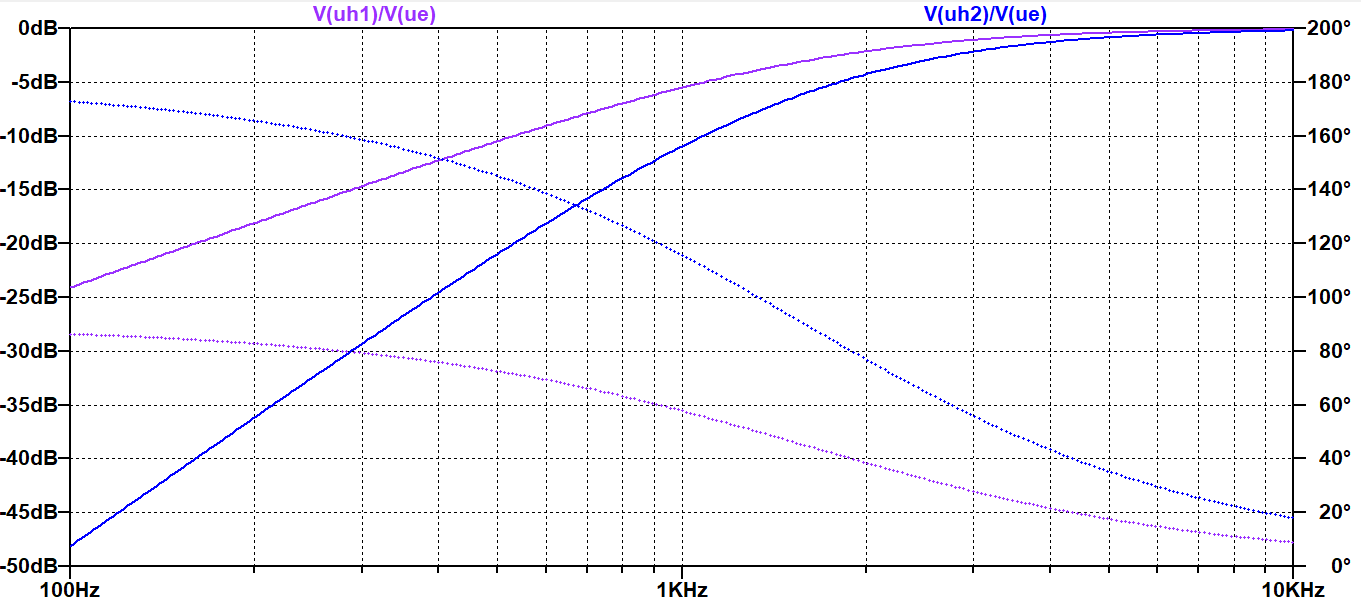
\includegraphics[width=16cm]{./pictures/Hochpass_Bode}
    \caption{Bodediagram des Hochpasses}
    \label{fig:HochpassBode}
\end{figure}

Die blaue Kurve stellt den geamten Hochpass dar, die violette Kurve nur einen einfachen Hochpass. Somit erkennt man anhand der Steigung einen Hochpass der Ordnung 2.

\newpage
\begin{figure}[htb]
    \includegraphics[width=14cm]{./pictures/Tiefpass}
    \caption{Aufbau des Tiefpasses}
    \label{fig:Tiefpass}
\end{figure}

\begin{figure}[htb]
    \includegraphics[width=14cm]{./pictures/Aufbau/Tiefpass}
    \caption{Praktischer Aufbau des Tiefpasses (links)}
    \label{fig:TiefpassPraktisch}
\end{figure}

In der Aufgabenstellung wird zudem ein Tiefpass der Ordnung zwei gefordert. Diese Anforderung realisieren wir mittels zwei typischer RC-Tiefpässe. Diese sind über einen Spannungsfolger gekoppelt. Der gesamte Tiefpass ist mit einem weiteren Spannungsfolger vom weiteren Verlauf der Schaltung sicher in Hinsicht auf Rückkopplungen und unzulässiger Ströme abgetrennt.

Wir wählen für unsere Kondensatoren und Widerstände die analogen Werte zum Hochpass, da wir die selbe Grenzfrequenz anstreben und die Frequenzformel des Hochpasses analog für den Tiefpass gilt. Somit erhalten wir auch hier eine Grenzfrequenz von $1591.6Hz$.

\newpage
Die Übertragungsfunktion ergibt sich gleichermaßen aus der Spannungsteilerregel und dem Verhältnis $U_{t2}$ zu $U_{e}$:
\gleichung{
\begin{split}
&\frac{U_a}{U_e} = \frac{C}{((R+C)||C)+R}
\\
&R+C = R+\frac{1}{j \omega C} = R-j \frac{1}{\omega C}
\\
&(R+C)||C) = \frac{(-j \frac{1}{\omega C})(R-j \frac{1}{\omega C})}{(R-j \frac{1}{\omega C})-j \frac{1}{\omega C}}
\end{split}
}{}
\gleichung{
\begin{split}
\frac{C}{(R+C)||C)} &= \frac{-j \frac{1}{\omega C}}{\frac{(-j \frac{1}{\omega C})(R-j \frac{1}{\omega C})}{(R-j \frac{1}{\omega C})-j \frac{1}{\omega C}}+R}
\\
&= \frac{-j \frac{1}{\omega C}}{\frac{-j \frac{R}{\omega C} - \frac{1}{(\omega C)^2}}{R-j \frac{2}{\omega C}}+R}
\\
&= \frac{\omega CR-j\frac{2\omega C}{\omega C}}{1-jR\omega C+(\omega CR)^2-j\frac{2R(\omega C)^2}{\omega C}}
\\
&= \frac{\omega CR-2j}{1+(\omega CR)^2-3jR\omega C}
\end{split}
}{}
\gleichung{
U_{a}(f) = \frac{\omega CR-2j}{1+(\omega CR)^2-3jR\omega C} * U_{e}(f)
}{}

\newpage
\begin{figure}[htb]
    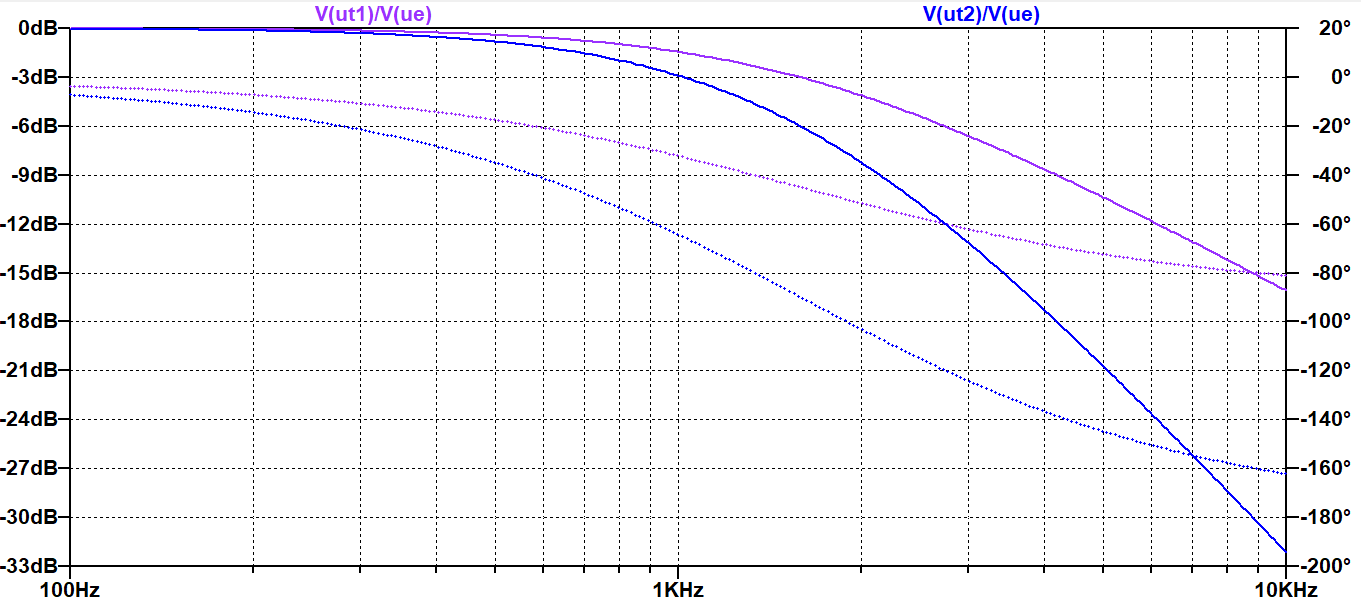
\includegraphics[width=16cm]{./pictures/Tiefpass_Bode}
    \caption{Bodediagram des Tiefpasses}
    \label{fig:TiefpassBode}
\end{figure}

Die blaue Kurve stellt den geamten Tiefpass dar, die violette Kurve nur einen einfachen Tiefpass. Somit erkennt man anhand der Steigung einen Tiefpass der Ordnung 2.

\subsubsection{Ergebnisse}

\begin{figure}[htb]
    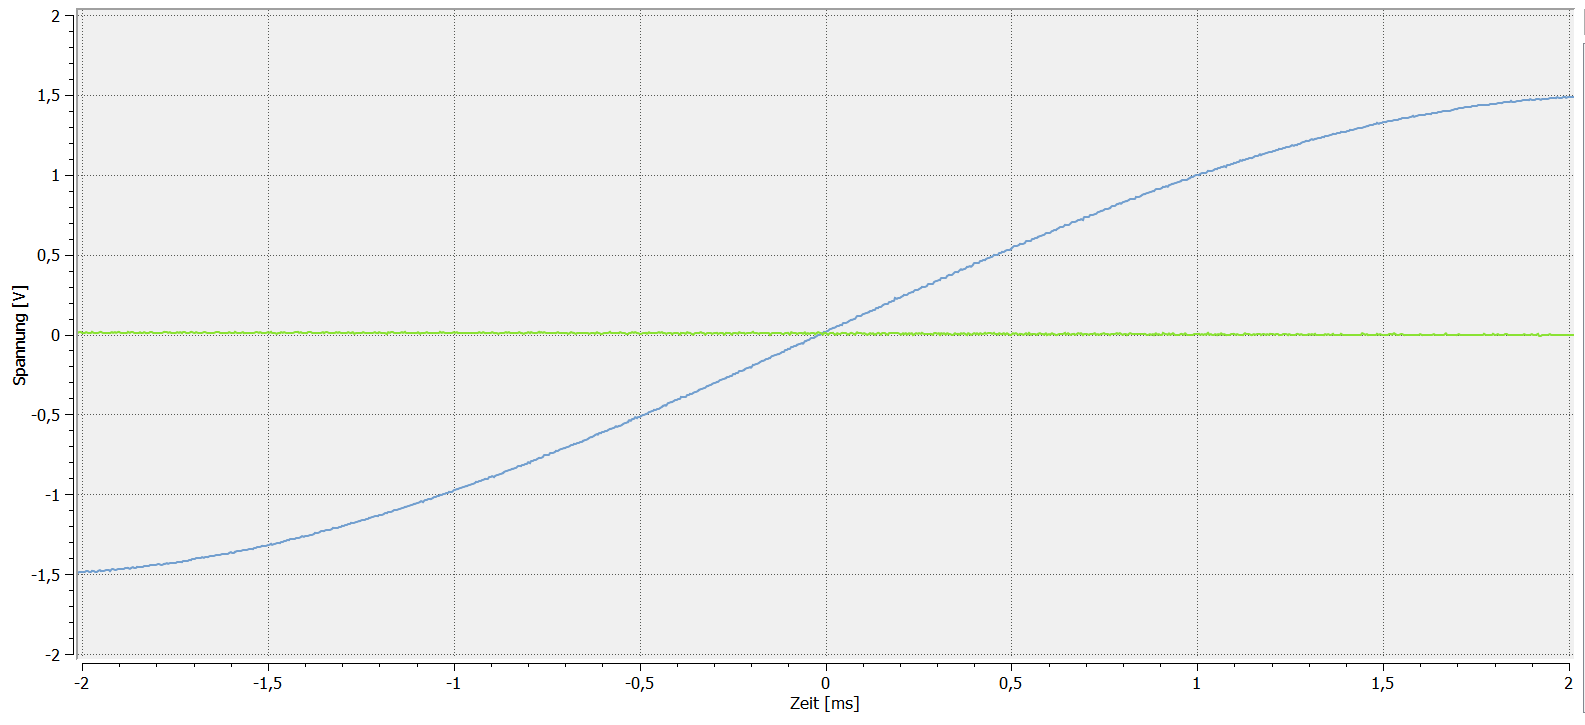
\includegraphics[width=16cm]{./pictures/Messungen/Hochpass_114}
    \caption{Praktische Messung des Hochpasses bei $f=114Hz$}
    \label{fig:Hochpass_114}
\end{figure}

\newpage
\begin{figure}[htb]
    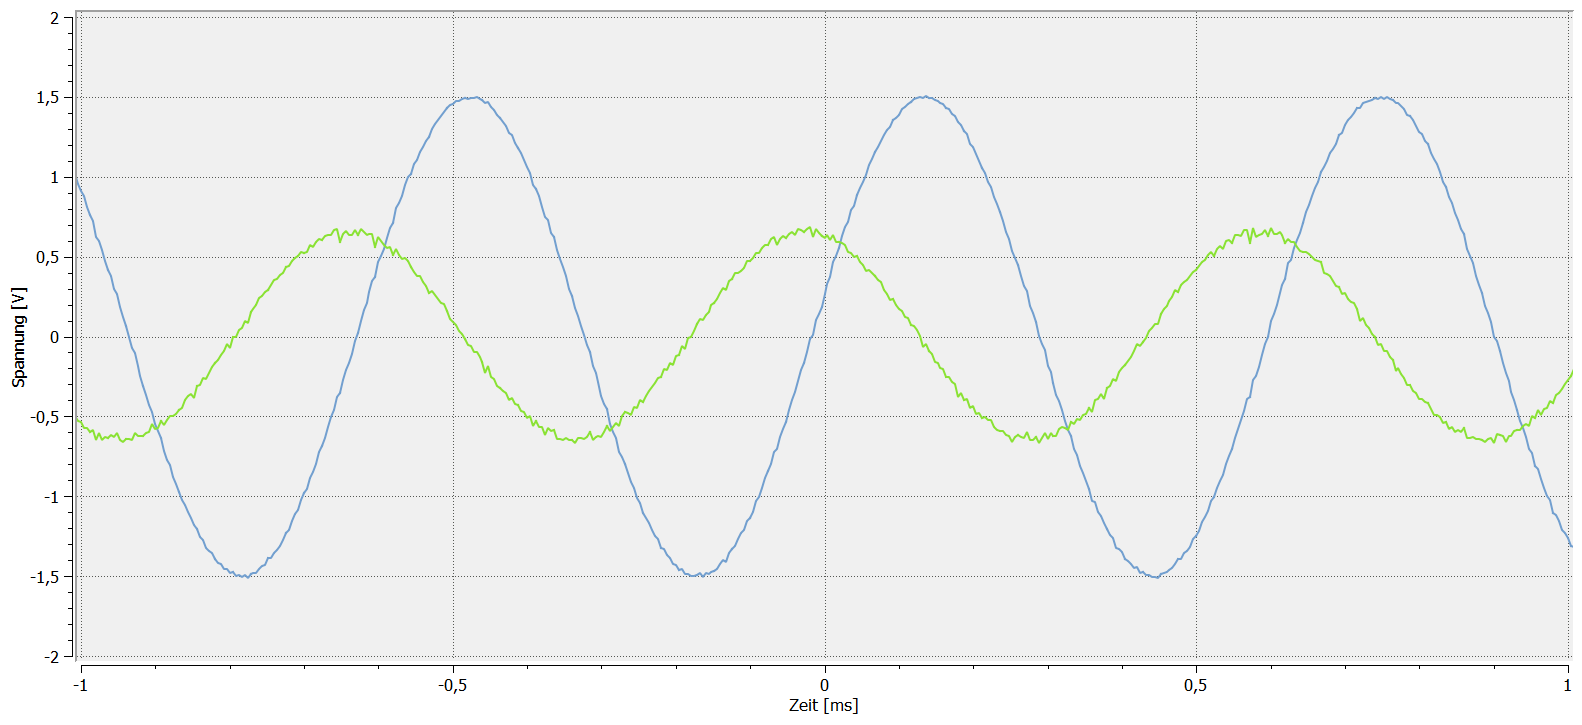
\includegraphics[width=13cm]{./pictures/Messungen/Hochpass_1,63k}
    \caption{Praktische Messung des Hochpasses bei $f=1.63kHz$}
    \label{fig:Hochpass_1,63k}
\end{figure}

\begin{figure}[htb]
    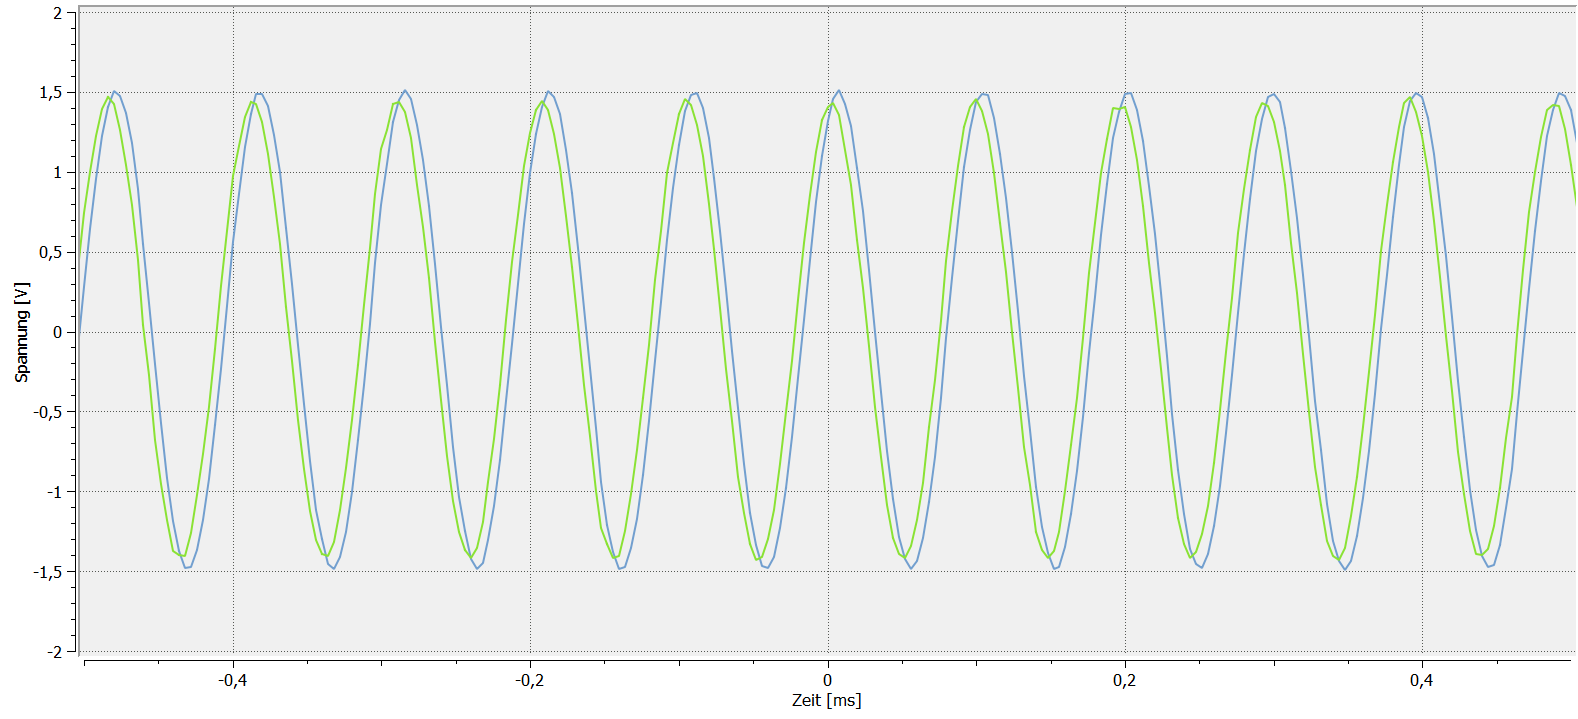
\includegraphics[width=13cm]{./pictures/Messungen/Hochpass_10k}
    \caption{Praktische Messung des Hochpasses bei $f=10kHz$}
    \label{fig:Hochpass_10k}
\end{figure}

~\\
Bei den Bildern des Hochpasses stellt die blaue Kurve unser Eingangssignal und die grüne Kurve unser Ausgangssignal dar.
\\
\\
Bei $f=114Hz$ (Abbildung \ref{fig:Hochpass_114}) wird die Eingangsspannung maximal gedämpft. Dies zeigt sich durch eine quasi konstante Ausgangsspannung bei 0V. Dieses Verhalten erwarten wir von einem Hochpass.
\\
\\
Bei $f=1.63kHz$ (Abbildung \ref{fig:Hochpass_1,63k}) (nah unserer Grenzfrequenz) wird die Eingangsspannung ca. halb gefämpft. Dies kann man an den Amplituden der sinusförmigen Spannungsbilder ablesen und ergibt sich aus den -3dB Verstärkung bei der Grenzfrequenz.
\\
\\
Bei $f=10kHz$ (Abbildung \ref{fig:Hochpass_10k}) wird die Eingangsspannung infinitisimal klein gefämpft. Hierbei überlappen sich Ein- und Ausgangsspannung. Wir erwarten dieses Verhalten bei einem Hochpass.

\newpage
\begin{figure}[htb]
    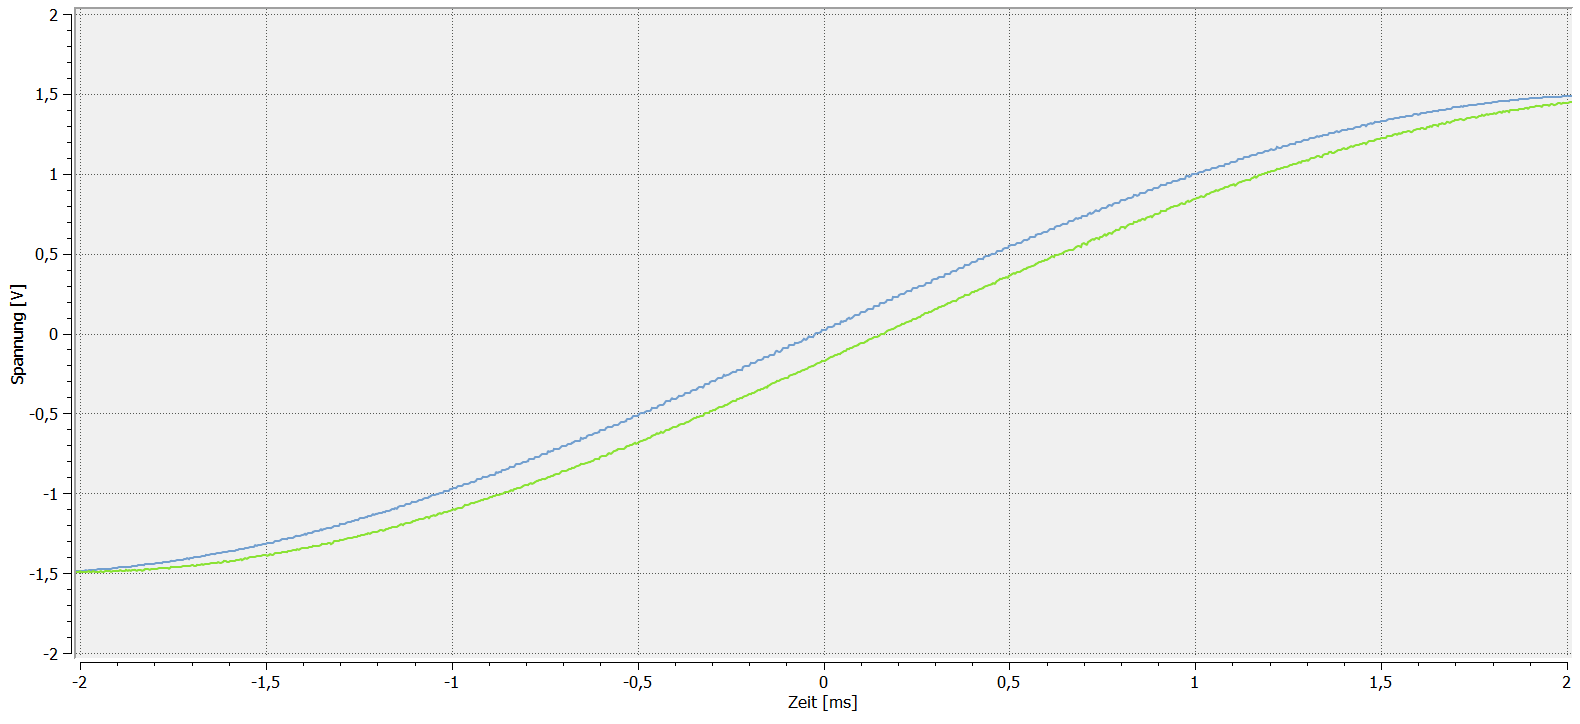
\includegraphics[width=16cm]{./pictures/Messungen/Tiefpass_114}
    \caption{Praktische Messung des Tiefpasses bei $f=114Hz$}
    \label{fig:Tiefpass_114}
\end{figure}

\begin{figure}[htb]
    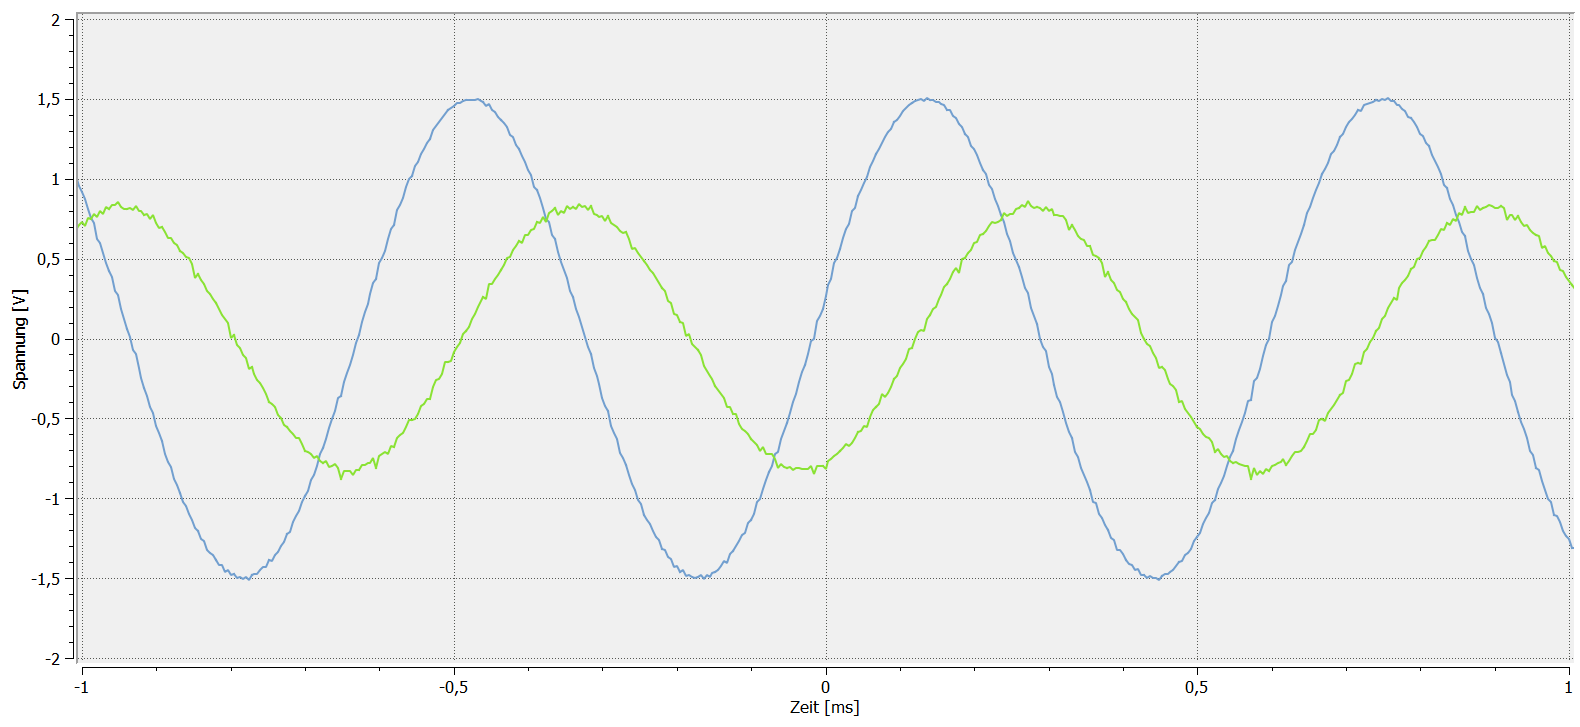
\includegraphics[width=16cm]{./pictures/Messungen/Tiefpass_1,63k}
    \caption{Praktische Messung des Tiefpasses bei $f=1.63kH$}
    \label{fig:Tiefpass_1,63k}
\end{figure}

\newpage
\begin{figure}[htb]
    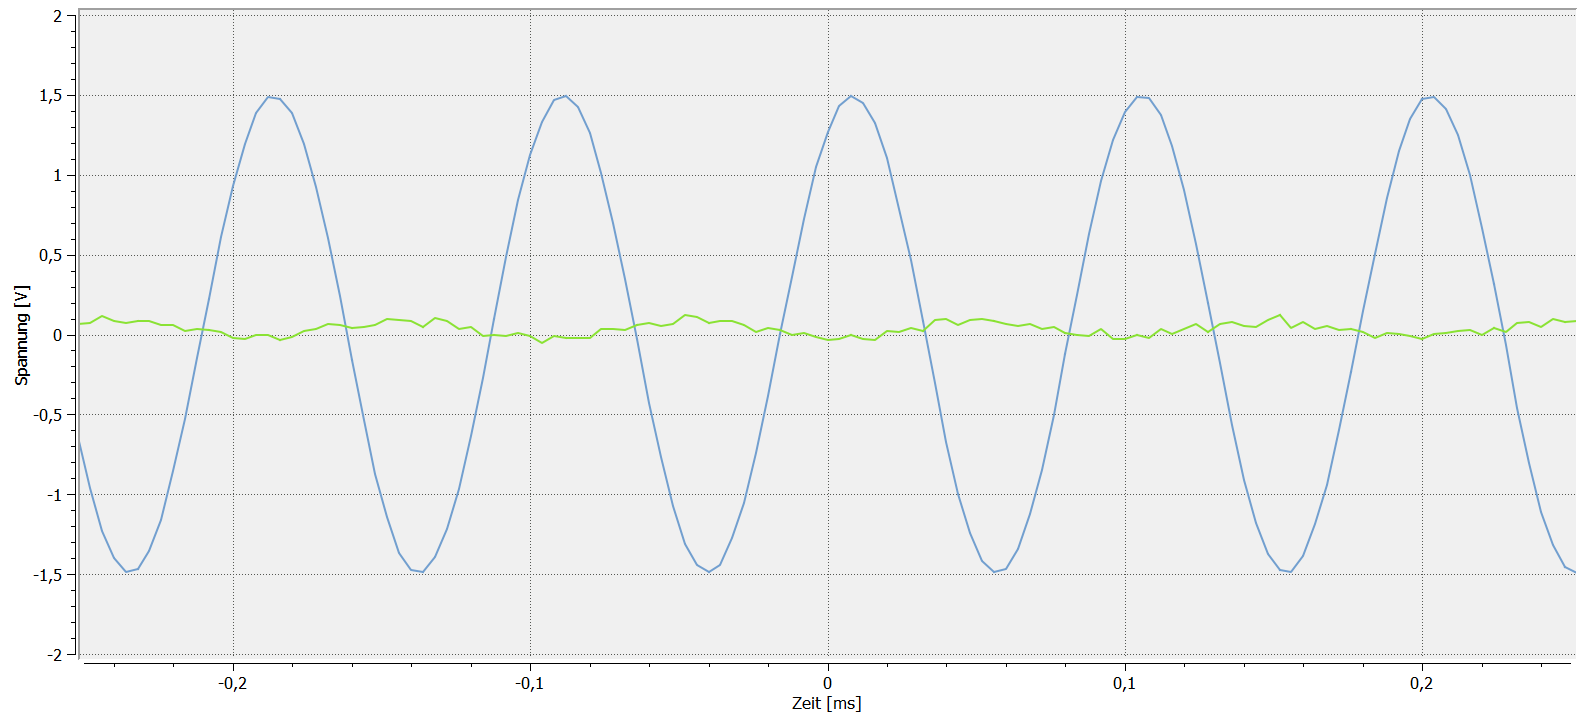
\includegraphics[width=13cm]{./pictures/Messungen/Tiefpass_10k}
    \caption{Praktische Messung des Tiefpasses bei $f=10kHz$}
    \label{fig:Tiefpass_10k}
\end{figure}

Bei den Bildern des Tiefpasses stellt die blaue Kurve unser Eingangssignal und die grüne Kurve unser Ausgangssignal dar.
\\
\\
Bei $f=114Hz$ (Abbildung \ref{fig:Tiefpass_114}) wird die Eingangsspannung infinitisimal klein gedämpft.  Die Amplitude des Ein- und Ausgangssignals ist dabei quasi identisch.
\\
\\
Bei $f=1.63kHz$ (Abbildung \ref{fig:Tiefpass_1,63k}) (nah unserer Grenzfrequenz) wird die Eingangsspannung ca. halb gefämpft. Dies kann man an den Amplituden der sinusförmigen Spannungsbilder ablesen und ergibt sich aus den -3dB Verstärkung bei der Grenzfrequenz. Dieses Spannungsbild ist dem des Hochpasses bei dieser Frequenz fast gleich.
\\
\\
Bei $f=10kHz$ (Abbildung \ref{fig:Tiefpass_10k}) wird die Eingangsspannung maximal gedämpft. Dies zeigt sich durch eine quasi konstante Ausgangsspannung bei 0V. Dieses Verhalten erwarten wir von einem Tiefpass.

\begin{figure}[htb]
    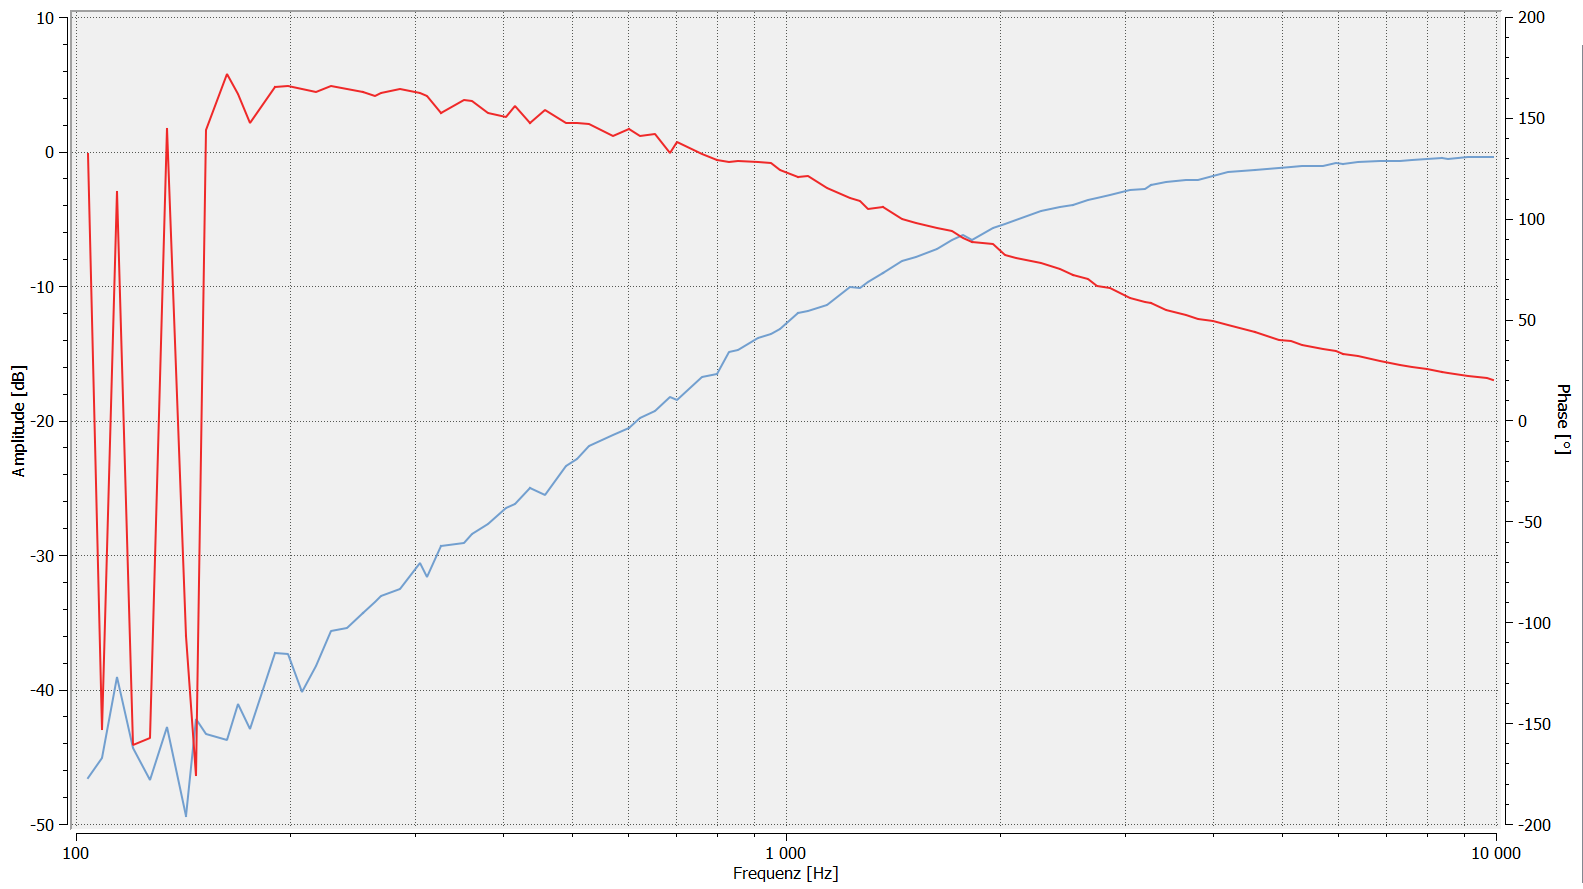
\includegraphics[width=13cm]{./pictures/Messungen/Hochpass_Bode_Test}
    \caption{Gemessenes Bode-Diagramm des Hochpasses}
    \label{fig:Hochpass_Bode_Test}
\end{figure}

\newpage

\begin{figure}[htb]
    \includegraphics[width=14cm]{./pictures/Messungen/tiefpass_Bode_Test}
    \caption{Gemessenes Bode-Diagramm des Tiefpasses}
    \label{fig:Tiefpass_Bode_Test}
\end{figure}

\subsubsection{Diskussion}

Unsere beiden Filterschaltungen funktionieren in der Praxis simultan zum simulierten Verhalten. Dabei treten zwar kleine Messungenauigkeiten auf, jedoch verhalten sich Phasen- und Amplitudengänge der Ausgangsspannungen wie erwartet für die konstruierten Filder. Der Hochpass filtert tiefe Frequenzen der Ausgangsspannung, der Tiefpass filtert hohe Frequenzen. 
\\
\\
Die gemessenen Bode-Diagramme des Hoch- und Tiefpasses stimmen mit den simulierten Diagrammen überein. Dabei treten beim Hochpass Messfehler bei sehr kleinen Frequenzen auf, aber der allgemeine Kurvenverlauf ist gleich. Die Messfehler kommen durch das Programm LenLab oder durch äußere Einflüsse zustande.

\newpage
\subsection{Addierschaltung}

\subsubsection{Materialien \& Methoden}

\begin{figure}[htb]
    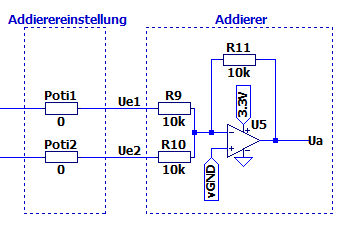
\includegraphics[width=14cm]{./pictures/Addierer}
    \caption{Addiererschaltung des Hoch- und Tiefpasses}
    \label{fig:Addierer}
\end{figure}

\begin{figure}[htb]
    \includegraphics[width=14cm]{./pictures/Aufbau/Gesamtschaltung}
    \caption{Praktischer Aufbau der Gesamtschaltung}
    \label{fig:GesamtschaltungPraktisch}
\end{figure}

\newpage
\begin{figure}[htb]
    \includegraphics[width=14cm]{./pictures/Aufbau/Ueberlagerung}
    \caption{Praktischer Aufbau der Überlagerungsschaltung}
    \label{fig:Überlagerung}
\end{figure}

\begin{figure}[htb]
    \includegraphics[width=16cm]{./pictures/Gesamtschaltung}
    \caption{Ausgangsspannung des Addierers}
    \label{fig:AddiererAusgangsspannung}
\end{figure}

Die ermittelte Kurve zeigt, dass einer der Filter eine negative Spannung erzeugt. Nach weiteren Simulationen mit Spice wurde festgestellt, dass der Tiefpass negative Spannungen erzeugt. Aufgrund dessen muss das Ausgangssignal des Tiefpasses invertiert werden, da sonst die Ausgangssignale nicht addiert, sonst subtrahiert werden.

\newpage

\begin{figure}[htb]
    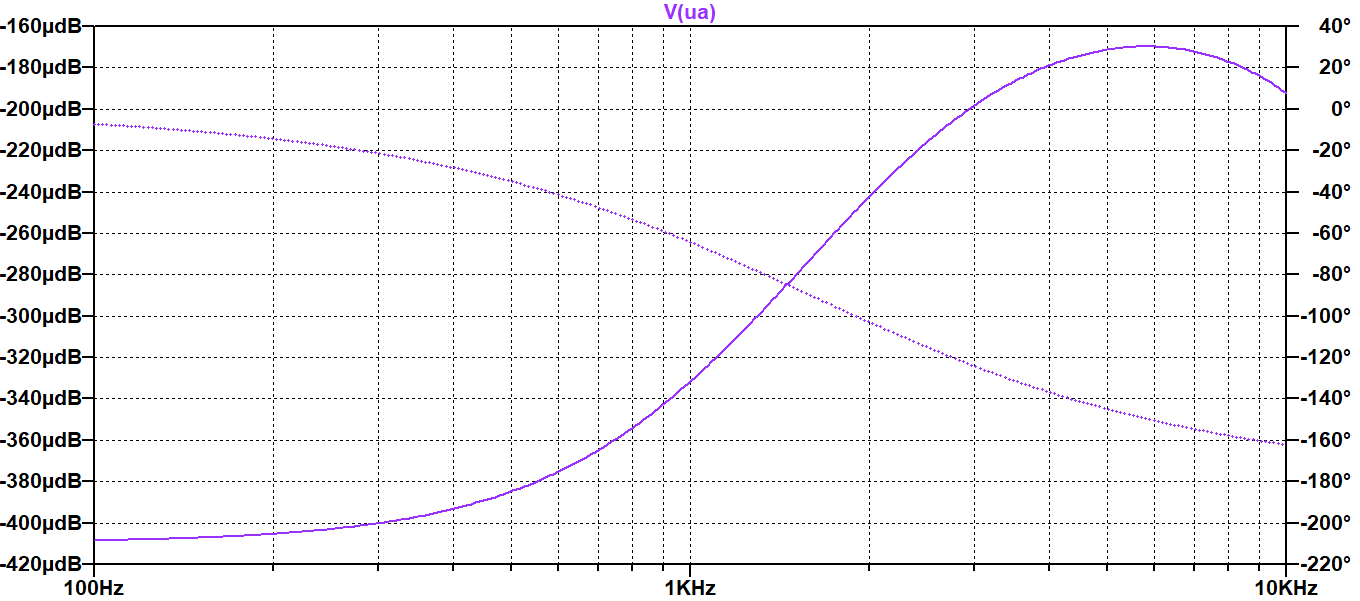
\includegraphics[width=16cm]{./pictures/Gesamtschaltung_Invertiert}
    \caption{Ausgangsspannung des Addierers mit invertiertem Tiefpass mit $R_1 = R_2 = 0$}
    \label{fig:AddiererAusgangsspannungInvertiert}
\end{figure}

Wir beobachten nun eine maximale Dämpfung des Signals bei 100Hz und Maximum bei ca 6000Hz. Die Funktion verläuft nun stetig ohne abrupte Änderung.
\\
\\
Einen solchen Filter bezeichnet man als 2-Band-Equalizer, da dieser aus einem kombinierten Hoch- und Tiefpass besteht und die jeweiligen Ausgangssignale des Hoch- und Tiefpasses einstellbar kombiniert werden können.

\begin{figure}[htb]
    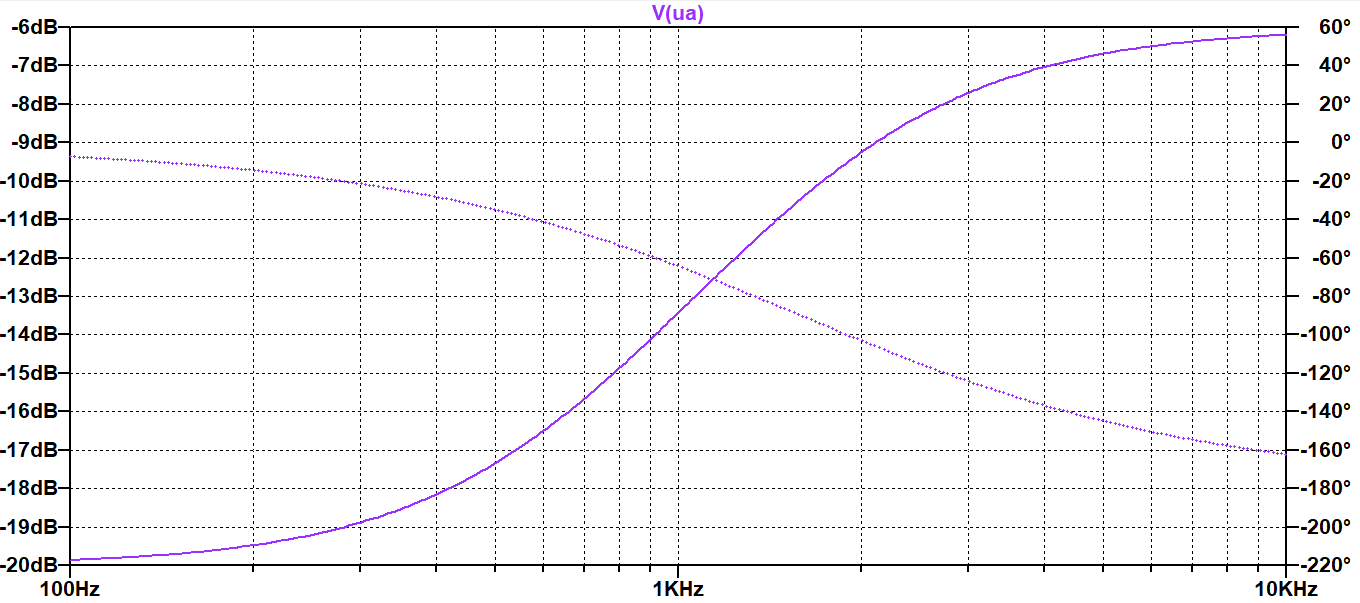
\includegraphics[width=16cm]{./pictures/Gesamtschaltung_Invertiert_10_90}
    \caption{Ausgangsspannung des Addierers mit invertiertem Tiefpass mit $R_1 = 10k\Omega$ und $R_2 = 90k\Omega$}
    \label{fig:AddiererAusgangsspannungInvertiert}
\end{figure}

\newpage

\begin{figure}[htb]
    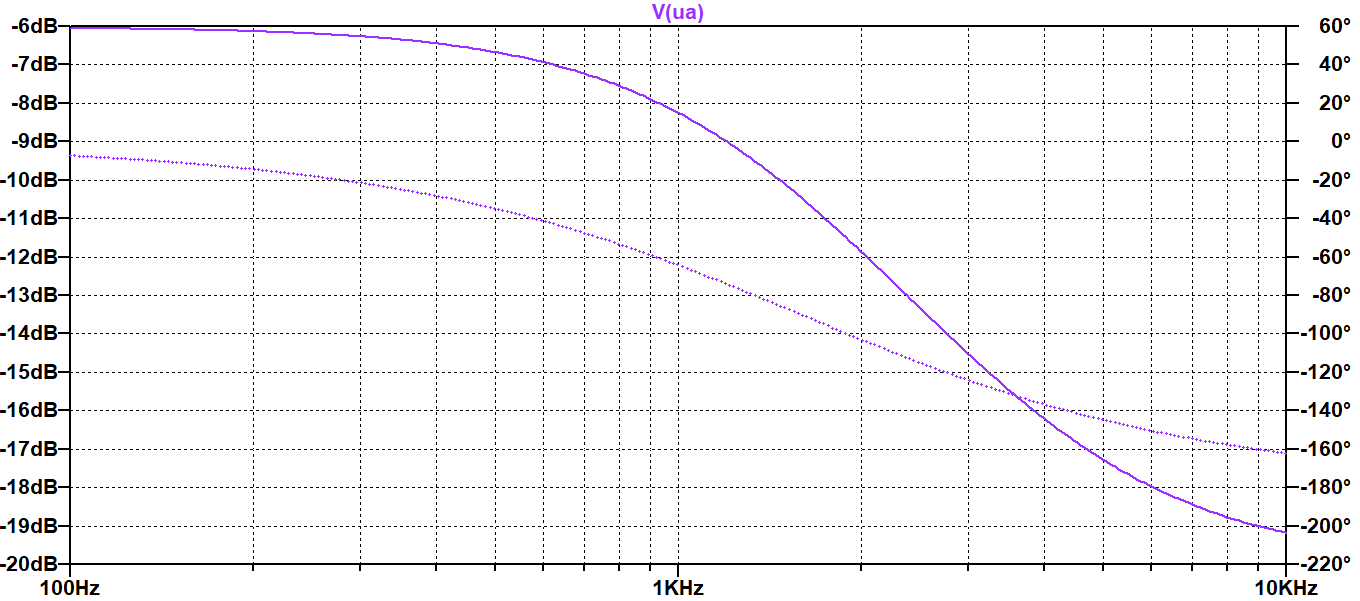
\includegraphics[width=16cm]{./pictures/Gesamtschaltung_Invertiert_90_10}
    \caption{Ausgangsspannung des Addierers mit invertiertem Tiefpass mit $R_1 = 90k\Omega$ und $R_2 = 10k\Omega$}
    \label{fig:AddiererAusgangsspannungInvertiert}
\end{figure}

Durch die Einstellungen an den Potentiometern lässt sich einstellen, welche Frequenzbereiche gedämpft werden sollen.

\subsubsection{Ergebnisse}

\begin{figure}[htb]
    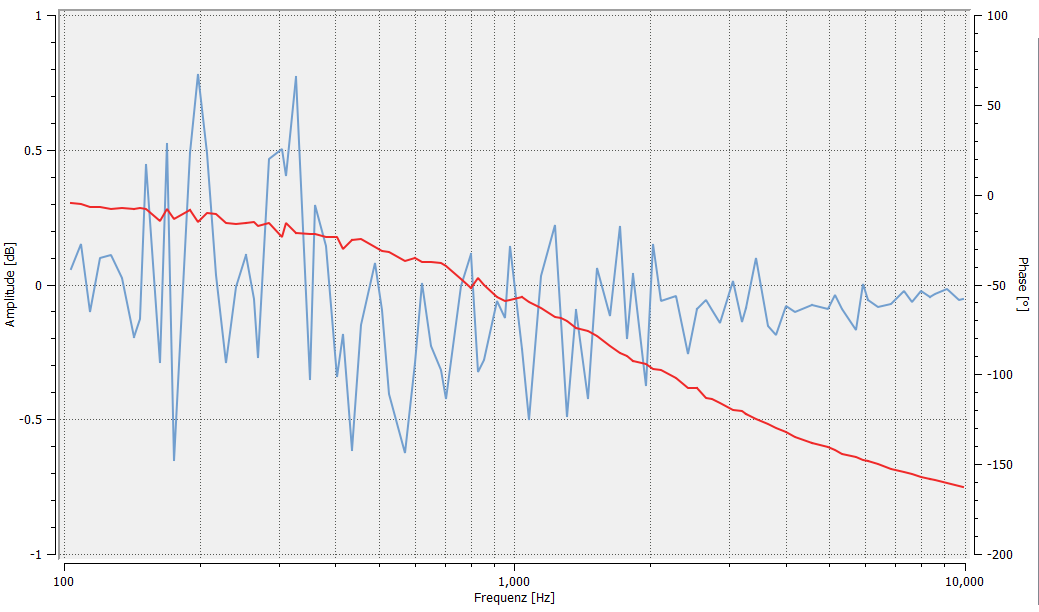
\includegraphics[width=16cm]{./pictures/Messungen/Gesamtschaltung_Test_0_0}
    \caption{Gemessene Ausgangsspannung mit $R_1 = 0\Omega$ und $R_2 = 0\Omega$}
    \label{fig:Gesamtschaltung_Test_0_0}
\end{figure}

\newpage

\begin{figure}[htb]
    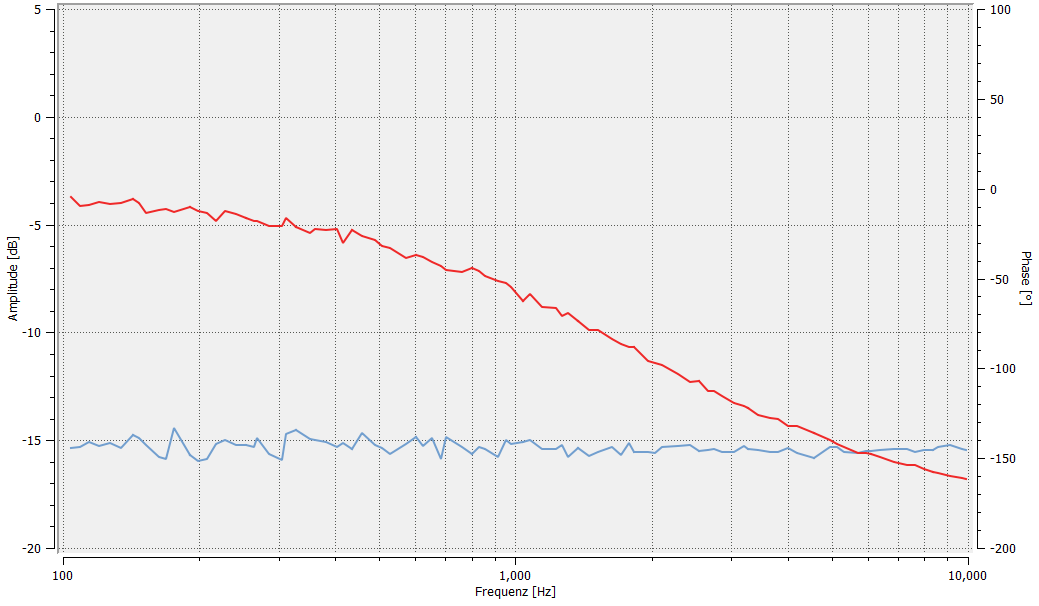
\includegraphics[width=16cm]{./pictures/Messungen/Gesamtschaltung_Test_50_50}
    \caption{Gemessene Ausgangsspannung mit $R_1 = 50k\Omega$ und $R_2 = 50k\Omega$}
    \label{fig:Gesamtschaltung_Test_50_50}
\end{figure}

\begin{figure}[htb]
    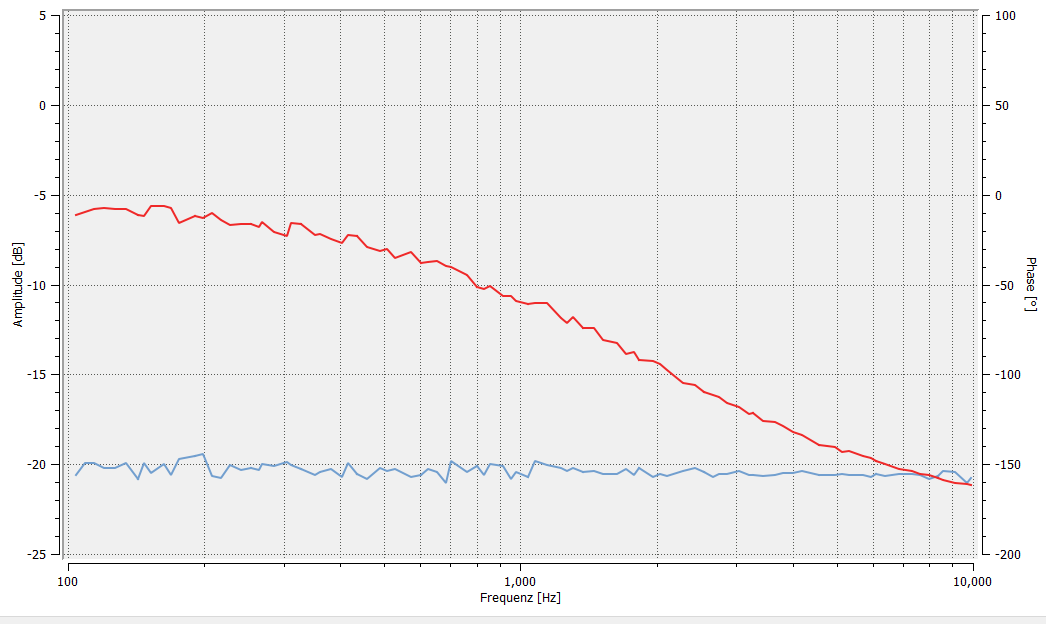
\includegraphics[width=16cm]{./pictures/Messungen/Gesamtschaltung_Test_100_100}
    \caption{Gemessene Ausgangsspannung mit $R_1 = 100k\Omega$ und $R_2 = 100k\Omega$}
    \label{fig:Gesamtschaltung_Test_100_100}
\end{figure}

\newpage

\begin{figure}[htb]
    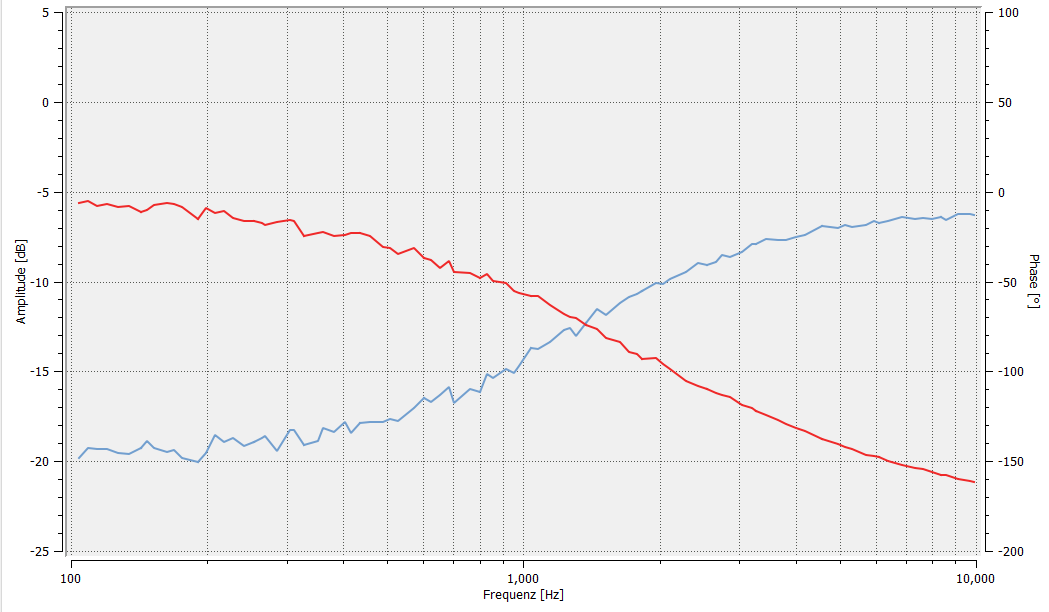
\includegraphics[width=16cm]{./pictures/Messungen/Gesamtschaltung_Test_10_90}
    \caption{Gemessene Ausgangsspannung mit $R_1 = 10k\Omega$ und $R_2 = 90k\Omega$}
    \label{fig:Gesamtschaltung_Test_10_90}
\end{figure}

\begin{figure}[htb]
    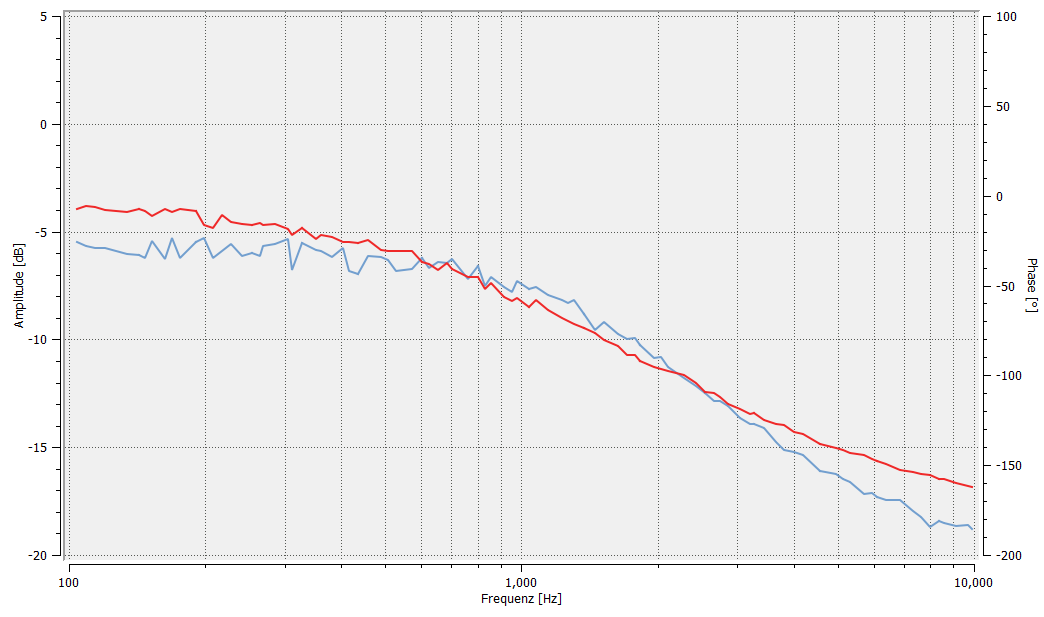
\includegraphics[width=16cm]{./pictures/Messungen/Gesamtschaltung_Test_90_10}
    \caption{Gemessene Ausgangsspannung mit $R_1 = 90k\Omega$ und $R_2 = 10k\Omega$}
    \label{fig:Gesamtschaltung_Test_90_10}
\end{figure}

Die blaue Kurve stellt den Amplitudeverlaug der Ausgangsspannung dar, die rote Kurve den phasenverlauf.

\newpage

\begin{figure}[htb]
    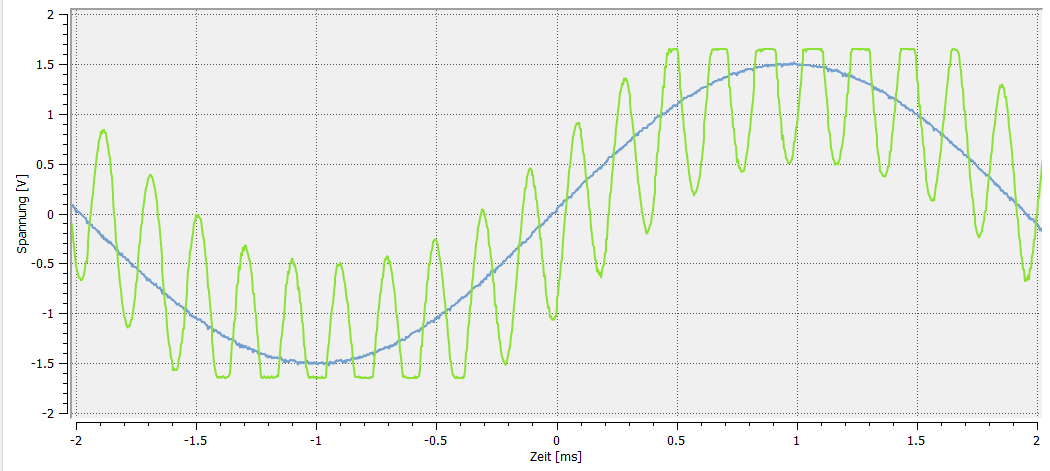
\includegraphics[width=16cm]{./pictures/Messungen/Ueberlagerung_100_0}
    \caption{Gemessene Ausgangsspannung bei $f_{1} = 254Hz$ und $f_{2} = 5080Hz$ mit $R_1 = 100k\Omega$ und $R_2 = 0\Omega$}
    \label{fig:Überlagerung_100_0}
\end{figure}

\begin{figure}[htb]
    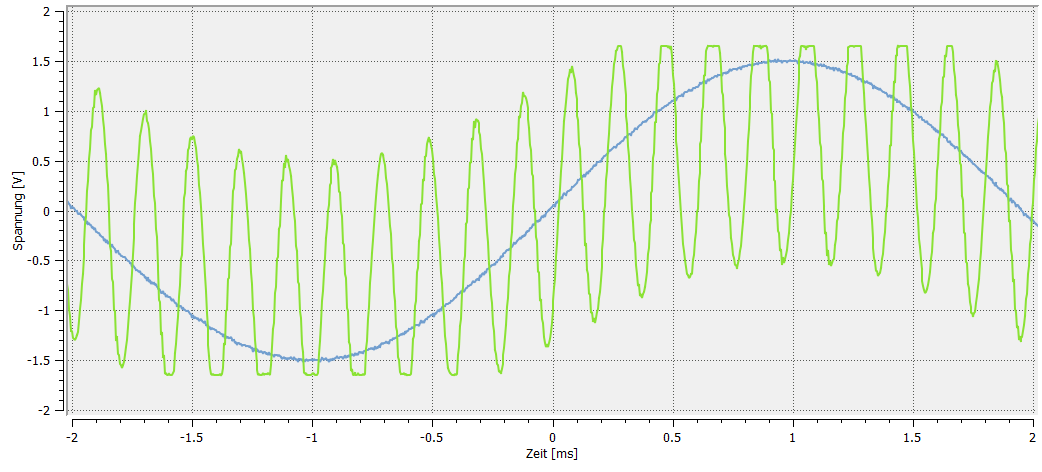
\includegraphics[width=16cm]{./pictures/Messungen/Ueberlagerung_0_100}
    \caption{Gemessene Ausgangsspannung bei $f_{1} = 254Hz$ und $f_{2} = 5080Hz$ mit $R_1 = 0\Omega$ und $R_2 = 100k\Omega$}
    \label{fig:Überlagerung_0_100}
\end{figure}

\subsubsection{Diskussion}

Unsere gemessenen Bildern mit unterschiedlichen Poti-Einstellungen ähneln den simulierten Werten stark. Bei Messungen mit $R_1 = 0\Omega$ und $R_2 = 0\Omega$ treten große Messfehler bezüglich der Spannung auf, die Phase ist deckungsgleich zu der der Simulation.
\\
\\
Bei gleichen Werten der beiden Potis lässt sich eine waagerechte Übertragungsfunktion erkennen. Dieses Verhalten haben wir erwartet, da die Signale des Hoch- und Tiefpasses äquivalent verrechnet werden.
\\
\\
Die Poti-Einstellungen bei $R_1 = 10k\Omega$ und $R_2 = 90k\Omega$ und bei $R_1 = 90k\Omega$ und $R_2 = 10k\Omega$ ergeben deckungsgleiche Verläufe der simulierten und gemessenen Ergebnissen. Im einen Fall werden tiefe Frequenzen gedämpft, im anderen werden hohe Frequenzen äquivalent gedämpft, wie wir es von unserem Equalizer erwarten.
\\
\\
\\
In den beiden Darstellungen stellt der blaue Graph die Eingansspannung mit 254Hz dar, die auf den Eingang des Equalizers gegeben wird und die grüne Kurve stellt das gemessene Ausgangssignal dar. Die Signale mit 254Hz und 5080Hz wurden mit den Anschlüssen des Spannungsteilers der virtuellen Masse verbunden.
\\
\\
Am Ausgangssignal ist eine Überlagerung der beiden Eingangssignale zu erkennen. Man erkennt eine 20-fach höhere Frequenz des Ausgangssignals im Vergleich zum Eingangssignal. Bei 1.65V wird die Spannung in LenLab abgeschnitten, da das DAC nur Spannungen bis 1.65V liefert. Bei hohen Hochpasswerten ($R_{1} = 100k\Omega$ und $R_{2} = 0\Omega$) ist die Amplitude der Ausgangsspannung geringer als die Ausgangsspannung bei hohen Tiefpasswerten ($R_{1} = 0\Omega$ und $R_{2} = 100k\Omega$).
\\
\\
Im Praxistest hat sich die Schaltung bewährt. Ein eingespeistes Musiksignal konnte mittels der Potis beeinflusst werden und somit hohe und Tiefe Tonfrequenzen reguliert werden. Auffällig war die schlechte Qualität (Rauschen) des Ausgangssignals. Wir schreiben dieses Rauschen der mangelnden Abschirmung und den schlechten Kontakten zwischen den einzelnen Bauteilen zu.

\newpage
\begin{sidewaysfigure}[htb]
    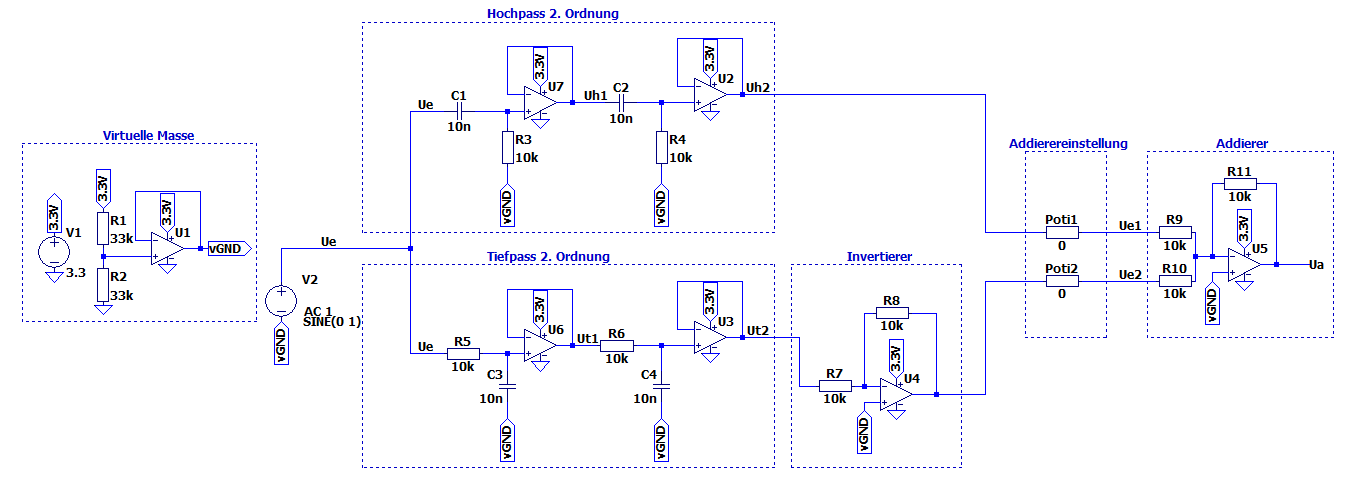
\includegraphics[width=22cm]{./pictures/Schaltung}
    \caption{Gesamtschaltung des Filters}
    \label{fig:Gesamtschaltung}
\end{sidewaysfigure}